% !TEX program = pdflatex
\documentclass[aspectratio=169, 10pt]{beamer}

%% ============================================================
%% PACKAGES
%% ============================================================
\usepackage[T1]{fontenc}
\usepackage{lmodern}
\usepackage{graphicx}
\usepackage{booktabs}
\usepackage{array}
\usepackage{tabularx}
\usepackage{colortbl}
\usepackage{tikz}
\usetikzlibrary{positioning, calc, arrows.meta, shapes.geometric, fit, shadows}
\usepackage[most]{tcolorbox}
\usepackage{fontawesome5}
\usepackage{hyperref}
\usepackage{pgfplots}
\pgfplotsset{compat=1.18}
\usepackage{multicol}
\usepackage{xcolor}
\usepackage{textcomp}
\usepackage{pifont}
\usepackage{fancyvrb}

\graphicspath{{figures/}{../Session1_Slides/figures/}}

%% ============================================================
%% COLOR DEFINITIONS (mirrored from Session 1)
%% ============================================================
\definecolor{UVMGreen}{HTML}{154734}
\definecolor{UVMGold}{HTML}{D4A84B}
\definecolor{SlateTeal}{HTML}{1B4D5C}
\definecolor{DeepCharcoal}{HTML}{2C3E50}
\definecolor{SoftCoral}{HTML}{C0534D}
\definecolor{CoolGray}{HTML}{8899A6}
\definecolor{PaleSage}{HTML}{EDF2F0}
\definecolor{LightGold}{HTML}{FDF6E3}
\definecolor{DarkSlate}{HTML}{0F2B36}
\definecolor{AccentBlue}{HTML}{3498DB}

%% ============================================================
%% BEAMER THEME SETUP
%% ============================================================
\setbeamercolor{structure}{fg=SlateTeal}
\setbeamercolor{normal text}{fg=DeepCharcoal}
\setbeamercolor{frametitle}{fg=SlateTeal}
\setbeamercolor{title}{fg=SlateTeal}
\setbeamercolor{subtitle}{fg=UVMGold}
\setbeamercolor{author}{fg=DeepCharcoal}
\setbeamercolor{date}{fg=CoolGray}
\setbeamercolor{institute}{fg=CoolGray}
\setbeamercolor{footline}{fg=CoolGray}
\setbeamercolor{block title}{fg=white, bg=SlateTeal}
\setbeamercolor{block body}{bg=PaleSage}
\setbeamercolor{alerted text}{fg=SoftCoral}
\setbeamercolor{item}{fg=SlateTeal}
\setbeamercolor{subitem}{fg=CoolGray}

\setbeamerfont{title}{size=\Large, series=\bfseries}
\setbeamerfont{subtitle}{size=\normalsize}
\setbeamerfont{frametitle}{size=\large, series=\bfseries}
\setbeamerfont{footline}{size=\tiny}

\setbeamertemplate{navigation symbols}{}

% Custom frame title
\setbeamertemplate{frametitle}{%
  \vskip14pt%
  \nointerlineskip%
  {\usebeamerfont{frametitle}\usebeamercolor[fg]{frametitle}\insertframetitle\par}%
  \vskip2pt%
  {\color{UVMGold}\rule{\textwidth}{1.2pt}}%
  \vskip3pt%
}

% Custom footline
\setbeamertemplate{footline}{%
  \begin{beamercolorbox}[wd=\paperwidth, ht=16pt, right, rightskip=1.5cm]{footline}%
    \usebeamerfont{footline}\insertframenumber\,/\,\inserttotalframenumber\vskip3pt%
  \end{beamercolorbox}%
}

% Itemize styles
\setbeamertemplate{itemize item}{\color{SlateTeal}\raisebox{0.15ex}{\small$\blacktriangleright$}}
\setbeamertemplate{itemize subitem}{\color{CoolGray}\raisebox{0.1ex}{\footnotesize$\bullet$}}

% Compact tcolorbox defaults (matches Session 1)
\tcbset{
  keybox/.style={
    colback=PaleSage, colframe=SlateTeal, boxrule=0.8pt, arc=3pt,
    left=6pt, right=6pt, top=4pt, bottom=4pt,
    fonttitle=\bfseries\small\color{white}, coltitle=white, colbacktitle=SlateTeal,
  },
  accentbox/.style={
    colback=LightGold, colframe=UVMGold, boxrule=0.8pt, arc=3pt,
    left=6pt, right=6pt, top=4pt, bottom=4pt,
  },
  quotebox/.style={
    colback=PaleSage, colframe=SlateTeal!50, boxrule=0.5pt, arc=2pt,
    left=8pt, right=8pt, top=4pt, bottom=4pt,
    borderline west={3pt}{0pt}{UVMGold},
  },
  promptbox/.style={
    colback=DarkSlate, colframe=DarkSlate, arc=3pt,
    left=7pt, right=7pt, top=4pt, bottom=4pt,
  },
  promptboxsm/.style={
    colback=DarkSlate, colframe=DarkSlate, arc=3pt,
    left=7pt, right=7pt, top=3pt, bottom=3pt,
  },
}

% Verbatim style for prompt boxes (white text on dark blue)
\fvset{fontsize=\tiny, fontfamily=tt, formatcom=\color{white}}

%% ============================================================
%% METADATA
%% ============================================================
\title{Agentic AI Bootcamp}
\subtitle{Applications: Teaching \& Research}
\author{Erkmen G. Aslim \and Emily Beam}
\institute{Department of Economics, University of Vermont}
\date{April 27, 2026}

\begin{document}

%% ====== SLIDE 1: TITLE ======
{
\setbeamertemplate{footline}{}
\begin{frame}[plain]
\begin{tikzpicture}[remember picture, overlay]
  \fill[SlateTeal] (current page.north west) rectangle (current page.south east);
  \fill[UVMGold] ([yshift=0.3cm]current page.center -| current page.west) rectangle ([yshift=0.25cm]current page.center -| current page.east);
  \node[anchor=center, text=white, font=\fontsize{28}{34}\bfseries\selectfont]
    at ([yshift=2.2cm]current page.center) {Agentic AI Bootcamp};
  \node[anchor=center, text=UVMGold, font=\fontsize{15}{20}\selectfont]
    at ([yshift=1.2cm]current page.center) {Applications: Teaching \& Research};
  \node[anchor=center, text=white, font=\large\bfseries]
    at ([yshift=-0.6cm]current page.center) {Erkmen G. Aslim \quad\&\quad Emily Beam};
  \node[anchor=center, text=PaleSage, font=\normalsize]
    at ([yshift=-1.3cm]current page.center) {Department of Economics, University of Vermont};
  \node[anchor=center, text=CoolGray!70!white, font=\small]
    at ([yshift=-2.2cm]current page.center) {Session 2 \quad$\cdot$\quad April 27, 2026 \quad$\cdot$\quad Old Mill A500};
  \node[anchor=center, text=UVMGold, font=\small\ttfamily]
    at ([yshift=-2.8cm]current page.center) {thinkingwithagents.github.io};
  \node[text=white, opacity=0.04, font=\fontsize{100}{100}\selectfont, anchor=center, rotate=-15]
    at ([xshift=5cm, yshift=1.5cm]current page.center) {\faRobot};
\end{tikzpicture}
\end{frame}
}

%% ====== SLIDE 2: RECAP & AGENDA ======
\begin{frame}{Where We Left Off \& Today's Plan}
\begin{columns}[T]
\begin{column}{0.47\textwidth}
\begin{tcolorbox}[keybox, title={\faHistory\quad From Session 1}]
\scriptsize
\begin{itemize}\setlength{\itemsep}{2pt}
  \item Agentic AI vs.\ chat AI
  \item Context window \& planning
  \item \texttt{CLAUDE.md}, \texttt{PLAN.md}, \texttt{SKILL.md}
  \item Permissions \& safety
  \item App 1 (live): website redesign
  \item App 2 (designed): \textbf{lecture-builder}
\end{itemize}
\end{tcolorbox}
\end{column}
\begin{column}{0.47\textwidth}
\begin{tcolorbox}[keybox, title={\faRocket\quad Today: Three Live Applications}]
\scriptsize
\begin{enumerate}\setlength{\itemsep}{2pt}
  \item \textbf{Lecture Builder} --- create the skill we designed last time, then run it on real papers
  \item \textbf{Research Brainstorm} --- stress-test an audience question live
  \item \textbf{Web Scraper} --- novel data on screen in 10 minutes
\end{enumerate}
\end{tcolorbox}
\end{column}
\end{columns}
\vfill
\begin{center}
\color{CoolGray}\small Each app is end-to-end: prompt $\rightarrow$ skill $\rightarrow$ output. Prompts are on the slides --- copy as we go.
\end{center}
\end{frame}

%% ====== SLIDE 3: SETUP -- INSTALL THE TOOLKIT ======
\begin{frame}[fragile]{Setup: Install Your Skill Toolkit}
\begin{columns}[T]
\begin{column}{0.50\textwidth}
\begin{tcolorbox}[keybox, title={\faDownload\quad Anthropic skills (one-time)}]
\scriptsize
\textbf{1. Add the marketplace:}\\
{\tiny\ttfamily /plugin marketplace add anthropics/skills}
\vskip3pt
\textbf{2. Install the document-skills bundle:}\\
{\tiny\ttfamily /plugin install \\\hspace*{1em}document-skills@anthropic-agent-skills}
\vskip3pt
{\raggedright\textbf{Gives you:} {\fontsize{6.5}{8}\selectfont\ttfamily pdf, docx, pptx, xlsx, frontend-design, skill-creator, algorithmic-art.}\par}
\end{tcolorbox}
\end{column}
\begin{column}{0.46\textwidth}
\begin{tcolorbox}[keybox, title={\faBoxes\quad Third-party skills via \texttt{npx}}]
\scriptsize
\textbf{Full economist pack:}\\
{\tiny\ttfamily npx skills add thinkingwithagents/skills}
\vskip3pt
\textbf{One skill at a time:}\\
{\tiny\ttfamily npx skills add thinkingwithagents/skills \\\hspace*{1em}-{}-skill research-brainstorm}
\vskip3pt
{\raggedright\textbf{Includes:} {\fontsize{6.5}{8}\selectfont\ttfamily research-brainstorm, find-data, academic-beamer-deck.}\par}
\end{tcolorbox}
\end{column}
\end{columns}
\vskip4pt
\pause
\begin{tcolorbox}[colback=SoftCoral!8, colframe=SoftCoral, boxrule=0.5pt, left=5pt, right=5pt, top=2pt, bottom=2pt, halign=center]
\scriptsize \faExclamationCircle\; \texttt{/skill-creator} is \textbf{not} bundled with Claude Code by default --- it ships inside \texttt{document-skills}. Install it before App 1.
\end{tcolorbox}
\end{frame}

%% ====== SECTION DIVIDER: APP 1 ======
{
\setbeamertemplate{footline}{}
\begin{frame}[plain, noframenumbering]
\begin{tikzpicture}[remember picture, overlay]
  \fill[SlateTeal] (current page.north west) rectangle (current page.south east);
  \node[text=white, font=\fontsize{22}{28}\bfseries\selectfont]
    at ([yshift=0.4cm]current page.center) {Application 1};
  \node[text=UVMGold, font=\normalsize]
    at ([yshift=-0.4cm]current page.center) {Lecture Builder Skill --- From Papers to a Lecture};
  \draw[UVMGold, line width=0.8pt] ([xshift=-2.5cm, yshift=0cm]current page.center) -- ([xshift=2.5cm, yshift=0cm]current page.center);
\end{tikzpicture}
\end{frame}
}

%% ====== SLIDE 5: WHERE WE LEFT OFF (the prompt) ======
\begin{frame}[fragile]{Where We Left Off --- The Skill Spec}
\begin{tcolorbox}[promptboxsm]
{\color{CoolGray}\fontsize{6}{7.5}\selectfont\ttfamily /skill-creator\\[2pt]
\color{white}\fontsize{6}{7.5}\selectfont\ttfamily
Create a skill called ``lecture-builder'' that converts academic documents into lecture materials. The skill should:\\[1pt]
1. Read documents in their entirety (PDF, DOCX, web pages) --- break reading into parts to avoid excessive token usage. Include a Python parsing script.\\[1pt]
2. Extract: key arguments, empirical findings, methodological details, discussion points, potential exam questions.\\[1pt]
3. Generate two outputs:\\
\quad a) Structured lecture notes (markdown) with section headers, key takeaways, discussion prompts\\
\quad b) A polished slide deck (draw on \textbackslash academic-beamer-deck or \textbackslash pptx) with clean visuals, one idea per slide\\[1pt]
4. Adapt tone for undergraduate vs.\ graduate audiences (configurable).\\[1pt]
Save SKILL.md + supporting files to .claude/skills/lecture-builder/.
}
\end{tcolorbox}
\vskip3pt
\begin{center}
{\scriptsize\color{CoolGray}\textit{Last week we wrote the spec. \textbf{\color{DeepCharcoal}Today we actually build the skill --- then run it.}}}
\end{center}
\end{frame}

%% ====== SLIDE 6: BUILDING THE SKILL FLOW ======
\begin{frame}{Building the Skill: \texttt{/skill-creator} Walkthrough}
\centering
\vskip4pt
\begin{tikzpicture}[
  stepbox/.style={
    draw=SlateTeal, fill=PaleSage, rounded corners=3pt,
    minimum width=2.3cm, minimum height=1.2cm,
    align=center, font=\tiny, text=DeepCharcoal
  },
  laststep/.style={
    draw=UVMGold, fill=LightGold, rounded corners=3pt,
    minimum width=2.3cm, minimum height=1.2cm,
    align=center, font=\tiny, text=DeepCharcoal
  },
  arr/.style={-{Stealth[length=3pt]}, SlateTeal, thick}
]
  \node[stepbox] (s1) at (0,0) {{\small\color{SlateTeal}\faTerminal}\\[1pt]\textbf{1. Invoke}\\\texttt{/skill-creator}};
  \node[stepbox, right=0.35cm of s1] (s2) {{\small\color{SlateTeal}\faPaste}\\[1pt]\textbf{2. Paste}\\the spec};
  \node[stepbox, right=0.35cm of s2] (s3) {{\small\color{SlateTeal}\faComments}\\[1pt]\textbf{3. Interview}\\4--6 design Qs};
  \node[stepbox, right=0.35cm of s3] (s4) {{\small\color{SlateTeal}\faCode}\\[1pt]\textbf{4. Skill writes}\\\texttt{SKILL.md} + script};
  \node[laststep, right=0.35cm of s4] (s5) {{\small\color{UVMGold}\faSave}\\[1pt]\textbf{5. Saved}\\\texttt{.claude/skills/}};
  \draw[arr] (s1) -- (s2);
  \draw[arr] (s2) -- (s3);
  \draw[arr] (s3) -- (s4);
  \draw[arr] (s4) -- (s5);
\end{tikzpicture}
\vskip12pt
\pause
\begin{tcolorbox}[accentbox, width=12cm, halign=center]
\scriptsize \texttt{/skill-creator} \textbf{interviews you}. Be ready to answer: name, audience, inputs, outputs, edge cases, where to save.
\end{tcolorbox}
\end{frame}

%% ====== SLIDE 7: ANATOMY OF THE LECTURE-BUILDER ======
\begin{frame}[fragile]{Anatomy of \texttt{lecture-builder}}
\begin{columns}[T]
\begin{column}{0.55\textwidth}
\centering
\vskip4pt
\begin{tikzpicture}[
  filebox/.style={
    draw=#1, fill=#1!8, rounded corners=2pt,
    minimum width=5.4cm, minimum height=0.55cm,
    align=left, font=\tiny\ttfamily, text=DeepCharcoal
  }
]
  \node[font=\scriptsize\bfseries, text=SlateTeal] at (0,1.9) {\faFolder\; \texttt{.claude/skills/lecture-builder/}};
  \node[filebox=SlateTeal] (skill) at (0,1.2) {\; SKILL.md \hfill {\normalfont\tiny\color{CoolGray}playbook}};
  \node[filebox=UVMGold] (parse) at (0,0.45) {\; parse\_document.py \hfill {\normalfont\tiny\color{CoolGray}PDF/DOCX reader}};
  \node[filebox=AccentBlue] (template) at (0,-0.3) {\; slide\_template.tex \hfill {\normalfont\tiny\color{CoolGray}UVM Beamer}};
  \node[filebox=SoftCoral] (notes) at (0,-1.05) {\; notes\_template.md \hfill {\normalfont\tiny\color{CoolGray}notes scaffold}};
\end{tikzpicture}
\end{column}
\begin{column}{0.42\textwidth}
\vskip4pt
\begin{tcolorbox}[keybox, title={What \texttt{SKILL.md} enforces}]
\scriptsize
\begin{itemize}\setlength{\itemsep}{1pt}
  \item Chunked reading $\rightarrow$ token control
  \item Mandatory citations from source PDFs
  \item Undergrad vs.\ grad tone toggle
  \item Dual output: notes + slides
  \item Reuses UVM color palette
\end{itemize}
\end{tcolorbox}
\end{column}
\end{columns}
\vskip4pt
\pause
\begin{tcolorbox}[quotebox, width=12cm]
\scriptsize Skills with Python scripts $>$ pure-markdown skills when tokens matter. The script reads; the LLM synthesizes.
\end{tcolorbox}
\end{frame}

%% ====== SLIDE 8: THE INPUT FOLDER ======
\begin{frame}{The Input Folder}
\begin{columns}[T]
\begin{column}{0.46\textwidth}
\centering
\vskip4pt
\begin{tikzpicture}[
  pdfbox/.style={
    draw=SlateTeal, fill=PaleSage, rounded corners=2pt,
    minimum width=5cm, minimum height=0.8cm,
    align=left, font=\scriptsize, text=DeepCharcoal
  },
  folderbox/.style={
    draw=UVMGold, fill=LightGold, rounded corners=3pt,
    minimum width=5.6cm, minimum height=0.55cm,
    align=center, font=\scriptsize\bfseries, text=DeepCharcoal
  }
]
  \node[folderbox] (fold) at (0,2.1) {\faFolderOpen\; \texttt{./inputs/}};
  \node[pdfbox] (p1) at (0,1.1) {\;\faFilePdf\; \texttt{gov\_thinktank\_ice\_arrests.pdf}\\[-1pt]\hspace*{1.4em}{\tiny\color{CoolGray} policy report}};
  \node[pdfbox] (p2) at (0,0.0) {\;\faFilePdf\; \texttt{ice\_enforcement\_report.pdf}\\[-1pt]\hspace*{1.4em}{\tiny\color{CoolGray} government brief}};
  \node[pdfbox] (p3) at (0,-1.1) {\;\faFilePdf\; \texttt{aslim\_paper.pdf}\\[-1pt]\hspace*{1.4em}{\tiny\color{CoolGray} academic working paper}};
  \draw[-{Stealth[length=3pt]}, CoolGray] (fold.south) -- ($(fold.south)+(0,-0.18)$);
\end{tikzpicture}
\end{column}
\begin{column}{0.50\textwidth}
\vskip4pt
\begin{tcolorbox}[accentbox]
\scriptsize
\textbf{Why this mix?}
\vskip3pt
\begin{itemize}\setlength{\itemsep}{1pt}
  \item Heterogeneous sources: \textbf{policy} + \textbf{government} + \textbf{academic}
  \item Forces the skill to harmonize tone, terminology, and evidence quality
  \item Mirrors how you'd actually build a lecture
\end{itemize}
\end{tcolorbox}
\vskip4pt
\pause
\begin{tcolorbox}[quotebox]
\scriptsize \textbf{Topic:} The labor and health consequences of ICE enforcement. Connects directly to ongoing research at UVM.
\end{tcolorbox}
\end{column}
\end{columns}
\end{frame}

%% ====== SLIDE 9: EXECUTION PROMPT ======
\begin{frame}[fragile]{The Execution Prompt}
\begin{tcolorbox}[promptboxsm]
{\color{CoolGray}\fontsize{5.5}{7}\selectfont\ttfamily /lecture-builder\\[2pt]
\color{white}\fontsize{5.5}{7}\selectfont\ttfamily
I have a folder ./inputs/ with: gov\_thinktank\_ice\_arrests.pdf,\\
ice\_enforcement\_report.pdf, aslim\_paper.pdf.\\[2pt]
Build a 50-minute undergraduate lecture on the labor and health\\
consequences of ICE enforcement. Audience: junior/senior econ majors\\
who have taken intermediate micro and one applied econometrics class.\\[2pt]
Outputs to ./outputs/:\\
\hspace*{1em}1) lecture\_notes.md --- sectioned notes with 5 key takeaways,\\
\hspace*{2em}4 discussion prompts, 3 candidate exam questions.\\
\hspace*{1em}2) lecture\_slides.tex --- Beamer deck (\textasciitilde 20 slides, 16:9). Use\\
\hspace*{2em}a clean academic palette --- default UVM (deep green / gold) or ask\\
\hspace*{2em}me. In-text citations to all three source PDFs.\\[2pt]
Be conservative with tokens: parse each PDF in chunks via\\
parse\_document.py, summarize per-section, then synthesize.
}
\end{tcolorbox}
\vskip3pt
\begin{center}
{\scriptsize\color{CoolGray}\textit{Audience spec + output spec + token discipline. Skills work better when the prompt is concrete.}}
\end{center}
\end{frame}

%% ====== SLIDE 10: EXPECTED OUTPUT ======
\begin{frame}{Expected Output (Live Demo Running)}
\centering
\vskip2pt
\begin{tcolorbox}[accentbox, width=11cm, halign=center, top=3pt, bottom=3pt]
\scriptsize \faPlay\quad Live demo running in the background --- final files appear by the end of this section
\end{tcolorbox}
\vskip6pt
\begin{tikzpicture}[
  doc/.style={
    draw=CoolGray!50, fill=white, rounded corners=2pt,
    minimum width=5cm, minimum height=4cm, align=left, font=\tiny,
    inner sep=4pt
  }
]
  \node[doc] (notes) at (-3.2,0) {%
    \textbf{lecture\_notes.md}\\[2pt]
    \rule{4.4cm}{0.3pt}\\[1pt]
    {\color{SlateTeal}\bfseries\# 1. The setting}\\
    Recent expansions of interior immigration\\
    enforcement\ldots\\[1pt]
    {\color{SlateTeal}\bfseries\# 2. Identification strategy}\\
    287(g) rollout as a staggered DiD\ldots\\[1pt]
    {\color{SlateTeal}\bfseries\# 3. Findings}\\
    Aslim et al.\ document\ldots\\[1pt]
    {\color{UVMGold}\bfseries\# Discussion prompts}\\
    1. Why might the effect on infant\\
    \hspace*{1em}health attenuate over time?\\[1pt]
    {\color{UVMGold}\bfseries\# Exam questions}\\
    1. Sketch the parallel-trends test\ldots
  };
  \node[doc] (slides) at (3.2,0) {%
    \textbf{lecture\_slides.tex}\\[2pt]
    \rule{4.4cm}{0.3pt}\\[1pt]
    {\color{CoolGray}\% 20 slides, 16:9}\\
    {\color{CoolGray}\% UVM palette}\\[2pt]
    \texttt{\textbackslash begin\{frame\}\{Setting\}}\\
    \hspace*{1em}\faChartBar\; ICE arrests timeline\\
    \texttt{\textbackslash end\{frame\}}\\[2pt]
    \texttt{\textbackslash begin\{frame\}\{Methods\}}\\
    \hspace*{1em}\faCogs\; staggered DiD\\
    \texttt{\textbackslash end\{frame\}}\\[2pt]
    \texttt{\textbackslash begin\{frame\}\{Results\}}\\
    \hspace*{1em}\faChartLine\; main effect\\
    \texttt{\textbackslash end\{frame\}}
  };
  \draw[-{Stealth[length=3pt]}, UVMGold, thick] (notes.east) -- (slides.west) node[midway, above, font=\tiny, text=CoolGray] {synthesizes};
\end{tikzpicture}
\end{frame}

%% ====== SLIDE 11: WHAT JUST HAPPENED ======
\begin{frame}{What Just Happened (Under the Hood)}
\centering
\vskip4pt

\begin{tikzpicture}[
  stage/.style={
    draw=SlateTeal, fill=PaleSage, rounded corners=4pt,
    minimum width=3cm, minimum height=1.6cm,
    align=center, font=\scriptsize, text=DeepCharcoal
  },
  arr/.style={-{Stealth[length=4pt]}, UVMGold, thick}
]
  \node<1->[stage] (read) at (-4.8,0)
    {{\large\color{SlateTeal}\faFilePdf}\\[2pt]\textbf{Read in chunks}\\{\tiny parse\_document.py}};
  \node<2->[stage] (synth) at (0,0)
    {{\large\color{SlateTeal}\faBrain}\\[2pt]\textbf{Synthesize}\\{\tiny LLM does the writing}};
  \node<3->[stage] (render) at (4.8,0)
    {{\large\color{SlateTeal}\faPalette}\\[2pt]\textbf{Render}\\{\tiny notes + Beamer .tex}};
  \draw<2->[arr] (read) -- (synth);
  \draw<3->[arr] (synth) -- (render);
\end{tikzpicture}
\vskip12pt
\onslide<4->{%
\begin{tcolorbox}[quotebox, width=11cm]
\scriptsize \textbf{This skill is reusable.} Swap the input folder, swap the topic, swap the audience --- get a new lecture in minutes. Build once, deploy forever.
\end{tcolorbox}%
}
\end{frame}

%% ====== SECTION DIVIDER: APP 2 ======
{
\setbeamertemplate{footline}{}
\begin{frame}[plain, noframenumbering]
\begin{tikzpicture}[remember picture, overlay]
  \fill[SlateTeal] (current page.north west) rectangle (current page.south east);
  \node[text=white, font=\fontsize{22}{28}\bfseries\selectfont]
    at ([yshift=0.4cm]current page.center) {Application 2};
  \node[text=UVMGold, font=\normalsize]
    at ([yshift=-0.4cm]current page.center) {\texttt{/research-brainstorm} --- Stress-Test a Research Idea};
  \draw[UVMGold, line width=0.8pt] ([xshift=-2.5cm, yshift=0cm]current page.center) -- ([xshift=2.5cm, yshift=0cm]current page.center);
\end{tikzpicture}
\end{frame}
}

%% ====== SLIDE 13: WHAT THE BRIEF CONTAINS ======
\begin{frame}{What the Research Brief Contains}
\begin{columns}[T]
\begin{column}{0.55\textwidth}
\begin{tcolorbox}[keybox, title={\faFile\quad Brief sections}, width=\textwidth]
\scriptsize
\begin{itemize}\setlength{\itemsep}{1pt}
  \item \textbf{The question} --- structured: unit, population, treatment, outcome, comparison, setting
  \item \textbf{Closest related work} --- 3--6 cites with sharp delta
  \item \textbf{Contribution type} --- setting / identification / reframing / measurement / mechanism / policy
  \item \textbf{The strongest objection} --- one paragraph, unvarnished
  \item \textbf{Alternative framings} --- 2--3 pivots
  \item \textbf{Feasibility} --- data, identification, power, timeline, fatal risks
  \item \textbf{Next concrete step}
\end{itemize}
\end{tcolorbox}
\end{column}
\begin{column}{0.42\textwidth}
\vskip2pt
\begin{tcolorbox}[accentbox]
\scriptsize
\textbf{Saved to:}\\
{\tiny\ttfamily research\_briefs/YYYY-MM-DD-{slug}.md}
\vskip4pt
Markdown so it lives next to your other notes. Re-openable, editable, citeable in your own write-ups.
\end{tcolorbox}
\vskip6pt
\pause
\begin{tcolorbox}[quotebox]
\scriptsize \textit{The conversation is great.\\ The artifact is what you keep.}
\end{tcolorbox}
\end{column}
\end{columns}
\end{frame}

%% ====== SLIDE 16: INSTALLING IT ======
\begin{frame}[fragile]{Installing \texttt{/research-brainstorm}}
\begin{columns}[T]
\begin{column}{0.48\textwidth}
\begin{tcolorbox}[keybox, title={\faCubes\quad Full economist pack}]
\scriptsize
{\tiny\ttfamily npx skills add\\\hspace*{1em}thinkingwithagents/skills}
\vskip4pt
Installs the full pack in one go. Today we use: {\fontsize{6.5}{8}\selectfont\ttfamily research-brainstorm, find-data, academic-beamer-deck.}
\end{tcolorbox}
\end{column}
\begin{column}{0.48\textwidth}
\begin{tcolorbox}[keybox, title={\faPuzzlePiece\quad One skill at a time}]
\scriptsize
{\tiny\ttfamily npx skills add\\\hspace*{1em}thinkingwithagents/skills\\\hspace*{1em}-{}-skill research-brainstorm}
\vskip4pt
Mix-and-match per project. Lighter footprint when you only need one.
\end{tcolorbox}
\end{column}
\end{columns}
\vskip6pt
\pause
\begin{tcolorbox}[accentbox, width=12cm, halign=center, top=3pt, bottom=3pt]
\scriptsize Same \texttt{npx skills} mechanism works for any GitHub-hosted skill repo. \textbf{Build your own pack and share it with your coauthors.}
\end{tcolorbox}
\end{frame}

%% ====== SLIDE 17: LIVE DEMO -- BRING ME A QUESTION ======
\begin{frame}{Live Demo: Hand Me a Question}
\centering
\vskip4pt
\begin{tcolorbox}[colback=SlateTeal, colframe=SlateTeal, arc=4pt, width=11cm, halign=center, top=8pt, bottom=8pt]
{\color{white}\Large\bfseries Audience:}\\[3pt]
{\color{UVMGold}\large\itshape hand me a half-formed research question.}
\end{tcolorbox}
\vskip10pt
\pause
\begin{columns}[T]
\begin{column}{0.31\textwidth}
\begin{tcolorbox}[quotebox, top=3pt, bottom=3pt]
\scriptsize\centering
\textbf{An effect}\\you suspect\\but can't yet measure
\end{tcolorbox}
\end{column}
\begin{column}{0.31\textwidth}
\begin{tcolorbox}[quotebox, top=3pt, bottom=3pt]
\scriptsize\centering
\textbf{A dataset}\\you have access to\\but haven't used
\end{tcolorbox}
\end{column}
\begin{column}{0.31\textwidth}
\begin{tcolorbox}[quotebox, top=3pt, bottom=3pt]
\scriptsize\centering
\textbf{A policy}\\you want\\to evaluate
\end{tcolorbox}
\end{column}
\end{columns}
\vskip8pt
{\scriptsize\color{CoolGray} Live: invoke \texttt{/research-brainstorm}, ride through the phases, walk away with a brief.}
\end{frame}

%% ====== SECTION DIVIDER: APP 3 ======
{
\setbeamertemplate{footline}{}
\begin{frame}[plain, noframenumbering]
\begin{tikzpicture}[remember picture, overlay]
  \fill[SlateTeal] (current page.north west) rectangle (current page.south east);
  \node[text=white, font=\fontsize{22}{28}\bfseries\selectfont]
    at ([yshift=0.4cm]current page.center) {Application 3};
  \node[text=UVMGold, font=\normalsize]
    at ([yshift=-0.4cm]current page.center) {Web Scraper --- From \texttt{/find-data} to a Live Visualization};
  \draw[UVMGold, line width=0.8pt] ([xshift=-2.5cm, yshift=0cm]current page.center) -- ([xshift=2.5cm, yshift=0cm]current page.center);
\end{tikzpicture}
\end{frame}
}

%% ====== SLIDE 18: APP 3 -- BRIEF FIND-DATA SLIDE ======
\begin{frame}{\texttt{/find-data} Picks NBER Working Papers}
\begin{columns}[T]
\begin{column}{0.46\textwidth}
\begin{tcolorbox}[keybox, title={\faSearch\quad \texttt{/find-data} in one line}]
\scriptsize
We hand it our constraints (applied-micro audience, 24+ months, scrape-able, time-series + cross-section). It scans repositories and surfaces a source.
\vskip3pt
\textbf{Today's pick:} NBER working papers.
\end{tcolorbox}
\end{column}
\begin{column}{0.50\textwidth}
\begin{tcolorbox}[accentbox]
\scriptsize
\textbf{Why NBER:} every economist cares; clean HTML; rich JEL + affiliation cross-section; \textasciitilde 1{,}500 papers / year.
\vskip3pt
\textbf{URL:}\\
{\tiny\ttfamily nber.org/papers?page=N\&perPage=100\&sortBy=public\_date}
\vskip3pt
\textbf{Extract:} {\fontsize{6.5}{8}\selectfont\ttfamily nber\_number, title, authors, public\_date, primary\_jel\_code, affiliations.}
\end{tcolorbox}
\end{column}
\end{columns}
\vskip4pt
\begin{center}
{\scriptsize\color{CoolGray}\textit{Goal: novel data on the screen in under 10 minutes. Skip the buildup --- go straight to scraping.}}
\end{center}
\end{frame}

%% ====== SLIDE 19: INSPECT THE PAGE ======
\begin{frame}{Inspect Before You Prompt}
\centering
\vskip2pt
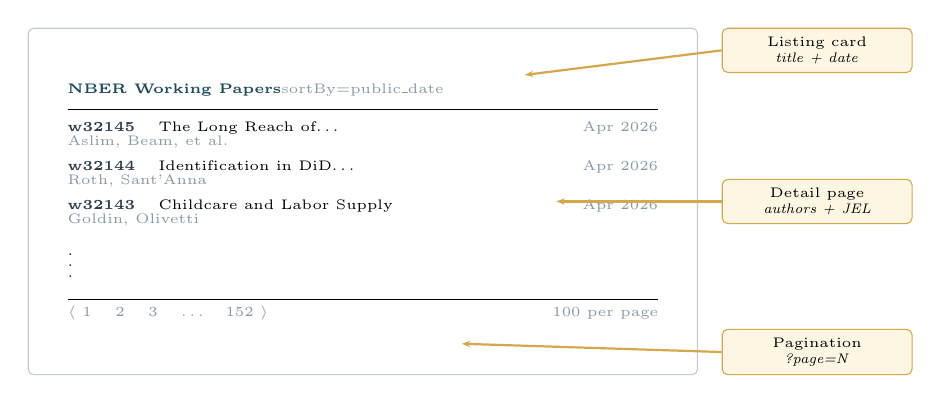
\begin{tikzpicture}[
  page/.style={
    draw=CoolGray!50, fill=white, rounded corners=2pt,
    minimum width=8.5cm, minimum height=4.4cm, font=\tiny,
    align=left, inner sep=6pt
  },
  callout/.style={
    draw=UVMGold, fill=LightGold, rounded corners=2pt,
    font=\tiny, align=center, inner sep=3pt
  },
  arr/.style={-{Stealth[length=3pt]}, UVMGold, thick}
]
  \node[page] (p) at (0,0) {%
    {\color{SlateTeal}\bfseries NBER Working Papers}\hfill {\tiny\color{CoolGray}sortBy=public\_date}\\
    \rule{7.5cm}{0.3pt}\\[2pt]
    {\color{DeepCharcoal}\bfseries w32145} \;\; The Long Reach of\ldots \hfill {\tiny\color{CoolGray}Apr 2026}\\[-1pt]
    {\tiny\color{CoolGray} Aslim, Beam, et al.}\\[3pt]
    {\color{DeepCharcoal}\bfseries w32144} \;\; Identification in DiD\ldots \hfill {\tiny\color{CoolGray}Apr 2026}\\[-1pt]
    {\tiny\color{CoolGray} Roth, Sant'Anna}\\[3pt]
    {\color{DeepCharcoal}\bfseries w32143} \;\; Childcare and Labor Supply\hfill {\tiny\color{CoolGray}Apr 2026}\\[-1pt]
    {\tiny\color{CoolGray} Goldin, Olivetti}\\[3pt]
    \vdots\\[2pt]
    \rule{7.5cm}{0.3pt}\\
    {\tiny\color{CoolGray}$\langle$ 1 \;\; 2 \;\; 3 \;\; \ldots \;\; 152 $\rangle$ \hfill 100 per page}
  };
  % Callouts
  \node[callout, right=0.3cm of p.north east, anchor=north west, text width=2.2cm] (c1) {Listing card\\\textit{title + date}};
  \node[callout, right=0.3cm of p.east, anchor=west, text width=2.2cm] (c2) {Detail page\\\textit{authors + JEL}};
  \node[callout, right=0.3cm of p.south east, anchor=south west, text width=2.2cm] (c3) {Pagination\\\textit{?page=N}};
  \draw[arr] (c1.west) -- ($(p.north east)+(-2.2,-0.6)$);
  \draw[arr] (c2.west) -- ($(p.east)+(-1.8,0)$);
  \draw[arr] (c3.west) -- ($(p.south east)+(-3,0.4)$);
\end{tikzpicture}
\vskip4pt
{\scriptsize\color{CoolGray}\textit{View-source first.} The agent writes better scrapers when you've already named the selectors.}
\end{frame}

%% ====== SLIDE 23: SCRAPING PROMPT ======
\begin{frame}[fragile]{The Scraping Prompt}
\begin{tcolorbox}[promptboxsm]
{\color{white}\fontsize{5.5}{7}\selectfont\ttfamily
Scrape NBER working papers for a teaching demo. Build a self-contained\\
Python script in ./scrape\_nber/ using uv:\\[2pt]
1.\;Fetch the most recent \textasciitilde 1{,}000 papers from\\
\hspace*{1.5em}nber.org/papers?page=N\&perPage=100\&sortBy=public\_date\\
\hspace*{1.5em}(paginate until 1{,}000 or cutoff 2024-01-01).\\
2.\;Extract: nber\_number, title, authors, public\_date, primary\\
\hspace*{1.5em}JEL code, affiliations (from detail page if needed).\\
3.\;Save to ./scrape\_nber/data/nber\_papers.csv.\\
4.\;Generate three PNGs to ./scrape\_nber/figures/:\\
\hspace*{1.5em}- papers\_per\_month.png \quad bars, last 24 months, UVM colors\\
\hspace*{1.5em}- top\_jel\_codes.png \quad top 15 primary JEL codes\\
\hspace*{1.5em}- top\_institutions.png \quad top 10 affiliations\\
5.\;Print 5-line stdout summary.\\[2pt]
Politeness: real-browser User-Agent; sleep 0.5s between fetches;\\
cache HTML to ./scrape\_nber/cache/ so re-runs are free.
}
\end{tcolorbox}
\end{frame}

%% ====== SLIDE 24: WHAT THE AGENT DOES ======
\begin{frame}{What Claude Does While We Keep Talking}
\begin{columns}[T]
\begin{column}{0.42\textwidth}
\centering
\vskip4pt
\begin{tikzpicture}[
  stage/.style={
    draw=CoolGray!50, fill=PaleSage, rounded corners=3pt,
    minimum width=4.2cm, minimum height=0.85cm,
    align=center, font=\scriptsize, text=DeepCharcoal
  },
  active/.style={
    draw=UVMGold, fill=LightGold, rounded corners=3pt,
    minimum width=4.2cm, minimum height=0.85cm,
    align=center, font=\scriptsize\bfseries, text=DeepCharcoal
  }
]
  \only<1>{\node[active] (s1) at (0,1.2) {\faSpinner\quad Fetching pages\ldots};}
  \only<2->{\node[stage] (s1) at (0,1.2) {\color{SlateTeal}\faCheck\quad Fetched 10 / 10 pages};}
  \only<-1>{\node[stage] (s2) at (0,0) {\color{CoolGray} Parsing\ldots};}
  \only<2>{\node[active] (s2) at (0,0) {\faSpinner\quad Parsing 1{,}000 records\ldots};}
  \only<3->{\node[stage] (s2) at (0,0) {\color{SlateTeal}\faCheck\quad Parsed 1{,}000 records};}
  \only<-2>{\node[stage] (s3) at (0,-1.2) {\color{CoolGray} Plotting\ldots};}
  \only<3>{\node[active] (s3) at (0,-1.2) {\faSpinner\quad Plotting 3 figures\ldots};}
  \only<4->{\node[stage] (s3) at (0,-1.2) {\color{SlateTeal}\faCheck\quad Wrote 3 PNGs};}
\end{tikzpicture}
\end{column}
\begin{column}{0.54\textwidth}
\vskip4pt
\begin{tcolorbox}[colback=DarkSlate, colframe=DarkSlate, arc=2pt, left=6pt, right=6pt, top=4pt, bottom=4pt]
{\color{white}\ttfamily\tiny
\$ uv run scrape\_nber/main.py\\[1pt]
{\color{CoolGray}[INFO]} fetching page 1/10 \ldots ok (98 papers)\\
{\color{CoolGray}[INFO]} fetching page 2/10 \ldots ok (100 papers)\\
{\color{CoolGray}[INFO]} \ldots\\
{\color{CoolGray}[INFO]} parsing JEL codes \ldots\\
{\color{CoolGray}[INFO]} saved data/nber\_papers.csv\\
{\color{CoolGray}[INFO]} writing figures/\ldots\\[3pt]
{\color{UVMGold}== Summary ==}\\
{\color{white}n\_papers: 1{,}000}\\
{\color{white}date range: 2024-04 to 2026-04}\\
{\color{white}top JEL: J (Labor)}\\
{\color{white}top affil: NBER, Harvard, MIT}
}
\end{tcolorbox}
\end{column}
\end{columns}
\vskip4pt
{\scriptsize\color{CoolGray}\textit{The terminal is a TV.} Let it run while you talk through what's coming.}
\end{frame}

%% ====== SLIDE 18: WHAT WE BUILT TODAY ======
\begin{frame}{What We Built Today}
\centering
\vskip4pt
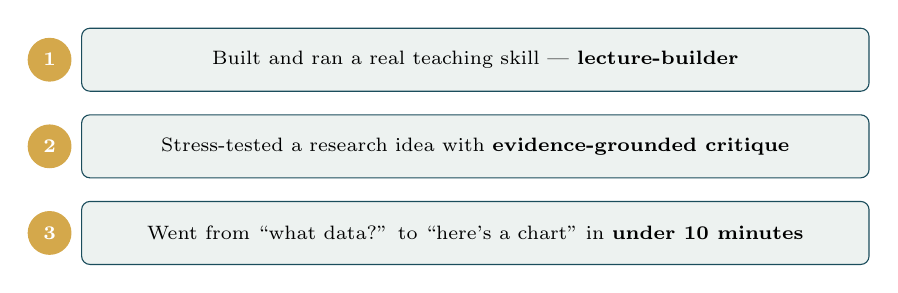
\begin{tikzpicture}[
  takeaway/.style={
    draw=SlateTeal, fill=PaleSage, rounded corners=3pt,
    minimum width=10cm, minimum height=0.8cm,
    align=center, font=\scriptsize
  }
]
  \node[circle, fill=UVMGold, text=white, font=\scriptsize\bfseries, minimum size=0.5cm] (n1) at (-5.7,1.3) {1};
  \node[takeaway, anchor=west] (t1) at (-5.3,1.3) {Built and ran a real teaching skill --- \textbf{lecture-builder}};
  \pause
  \node[circle, fill=UVMGold, text=white, font=\scriptsize\bfseries, minimum size=0.5cm] (n2) at (-5.7,0.2) {2};
  \node[takeaway, anchor=west] (t2) at (-5.3,0.2) {Stress-tested a research idea with \textbf{evidence-grounded critique}};
  \pause
  \node[circle, fill=UVMGold, text=white, font=\scriptsize\bfseries, minimum size=0.5cm] (n3) at (-5.7,-0.9) {3};
  \node[takeaway, anchor=west] (t3) at (-5.3,-0.9) {Went from ``what data?'' to ``here's a chart'' in \textbf{under 10 minutes}};
\end{tikzpicture}
\vskip12pt
\onslide<4->{%
\begin{tcolorbox}[accentbox, width=10cm, halign=center, top=3pt, bottom=3pt]
\small Three workflows. Three artifacts on disk. \textbf{All reusable.}
\end{tcolorbox}
}
\end{frame}

%% ====== SLIDE 19: THINKING WITH AGENTS PROMO (LAST) ======
{
\setbeamertemplate{footline}{}
\begin{frame}[plain]
\begin{tikzpicture}[remember picture, overlay]
  \fill[SlateTeal] (current page.north west) rectangle (current page.south east);
  \fill[UVMGold] ([yshift=0.3cm]current page.center -| current page.west) rectangle ([yshift=0.25cm]current page.center -| current page.east);
  \node[anchor=center, text=white, font=\fontsize{24}{30}\bfseries\selectfont]
    at ([yshift=2.2cm]current page.center) {Thinking With Agents};
  \node[anchor=center, text=UVMGold, font=\fontsize{14}{18}\selectfont]
    at ([yshift=1.3cm]current page.center) {Online sessions coming this summer};
  \node[anchor=center, text=white, font=\normalsize, text width=10cm, align=center]
    at ([yshift=-0.3cm]current page.center) {Workshops, deep-dives, and Q\&A on agentic AI for academic research --- built by economists, for economists and academics alike.};
  \node[anchor=center, text=PaleSage, font=\small]
    at ([yshift=-1.7cm]current page.center) {Stay tuned for dates and registration:};
  \node[anchor=center, text=UVMGold, font=\small\ttfamily]
    at ([yshift=-2.3cm]current page.center) {thinkingwithagents.github.io};
  \node[text=white, opacity=0.04, font=\fontsize{100}{100}\selectfont, anchor=center, rotate=15]
    at ([xshift=5cm, yshift=-1cm]current page.center) {\faBrain};
\end{tikzpicture}
\end{frame}
}

\end{document}
